% vim:ts=4:sw=4
% Copyright (c) 2014 Casper Ti. Vector
% Public domain.

\chapter{延迟环路PUF设计}\label{chap:dbrpuf}
在本章我们针对 BRPUF 进行改进,使 CRP 的统计分布趋于理想值。

\section{电路结构}\label{sec:dbrpuf_scheme}
从第\ref{chap:buildingmodel}章的讨论看出, BRPUF 输出分布在(0,1)几乎呈均匀分布,这是 PUF 设计所不愿意看到的,其根本原因在式\ref{eq:brmodel}中常数项是和式,环路结构使得每一个环路中与非门的延迟波动产生叠加,造成了最终输出均值较大波动,根据定理1,在工艺方差不变的前提下,输出分布方差退化为工艺方差的 N 倍(N为级数),故级数 N 越高, BRPUF 输出分布越差。

\textbf{定理1:}若 $ \beta_i, i=1,2,...,n $ 满足 $ \beta_i~N(\mu_0,\sigma_0) $,则 $ B=\sum\limits_{i=1}^{n}\beta_i~N(n\mu_0,\sqrt{n\sigma^2_0}) $。

由于 Strong PUF 要求,在保证 CRP 空间大小不变 ($ 2^N $)的情况下,必须改变激励作用的方式。
结合 BRPUF 环路结构和仲裁 PUF 的延迟路径选择结构,本文提出了如图\ref{fig:dbrpuf}所示的电路,称为``延迟环路PUF''( Delay-based Bistable Ring PUF, DBRPUF )。

\begin{figure}[htb]
\centering
\includegraphics[width=\linewidth]{dbrpuf}
\caption{延迟环路PUF电路示意图}
\label{fig:dbrpuf}
\end{figure}

如图\ref{fig:dbrpuf}所示,该结构由 $ N=2 $ 个单元构成,每个单元固定包含2个与非门和 $ K=4 $ 个双口交换器,其中交换器 $ 0\sim K-1 $ 由激励 $ c_0\sim c_2 $ 控制,最后一级交换器由 $ z_0=c_0\oplus c_1\oplus...\oplus c_{K-1}  $ 控制,使得最后一级交换器的底输出端口一定和顶与非门 I0 联接,而顶输出一定与底与非门 I1 相联接,因此每个单元有 $ K-1 $ 位激励输入,1位信号输入,1位信号输出和1位复位信号。N个单元输入输出连接成环路,在此结构中,由 $ 2N $ 个与非门组成了双稳态环路,激励信号 $ c_i $  控制每个与非门的延迟路径。

根据\ref{sec:brpufmodel}节理论,双稳环路的稳定态与环路中每一个与非门延迟相关,当 Rst 信号为低时,所有与非门被强制输出``1'',复位所有节点到高电平。激励C选定环路``S0(I0)--S0(I1)--S1(I0)--S1(I1)--S0(I0)''的连接路径,不同的路径使得信号从与非门 $ \text{I}_i $ 的输出到 $ \text{I}_{i+1} $ 的输入延时时间不同。
图\ref{fig:dbrpuf}中延迟可以看成与非门本征延迟和交换器延迟的累积,因此改变交换器状态即改变了环路中与非门的输入信号延迟时间,进而导致电路进入不同的稳态。
故该 PUF 结构的 CRP 共有 $ 2^{N(K-1)} $ 对。

\section{统计分析}\label{sec:dbrpuf_stat}
现在推导激励与响应的逻辑关系。

设第i个单元中顶与非门 I0 和底与非门 I1 的总延迟分别为 $ (Sr_i^T,Sf_i^T),(Sr_i^B,Sf_i^B) $,其中 $ Sr $ 代表总上升沿延迟, $ Sf $ 代表总下降沿延迟。
令信号从顶与非门I0输出的时刻为 $ p_0 $ ,底与非门I1输出的时刻为 $ q_0 $。每一级交换器j有4条路径,每条路径有上升延迟和下降延迟两个变量,用 $ (x_0^j,x_1^j,x_2^j,x_3^j) $ 表示4条路径的上升沿延迟,同理用 $ (y_0^j,y_1^j,y_2^j,y_3^j) $ 表示下降沿延迟。

首先考虑上跳沿的传输。仍然用{-1,1}表示逻辑上的{0,1},由交换器的逻辑关系可得每一级的递推式:
\begin{eqnarray}
\label{eq:dbr1}
p_{j+1}=\frac{1-c_j}{2}(p_j+x_0^j)+\frac{1+c_j}{2}(q_j+x_2^j) \\
\label{eq:dbr2}
q_{j+1}=\frac{1-c_j}{2}(q_j+x_3^j)+\frac{1+c_j}{2}(p_j+x_1^j)
\end{eqnarray}

两式相减得到类似于仲裁型PUF延时差的表达式:
\begin{equation}
\Delta_{j+1}=p_{j+1}-q_{j+1}=-\Delta_jc_j+\alpha_jc_j+\beta_j
\end{equation}

同理,式\ref{eq:dbr2}与\ref{eq:dbr2}相加得到:
\begin{equation}
S_{j+1}=p_{j+1}+q_{j+1}=S_j+\gamma_jc_j+\tau_j
\end{equation}

其中:
\begin{eqnarray}
\alpha_j=\frac{x_0^j-x_1^j-x_2^j+x_3^j}{2} \nonumber\\
\beta_j=\frac{x_0^j-x_1^j+x_2^j+x_3^j}{2} \nonumber\\
\gamma_j=\frac{x_0^j-x_1^j-x_2^j+x_3^j}{2} \nonumber\\
\tau_j=\frac{x_0^j+x_1^j+x_2^j+x_3^j}{2} \nonumber
\end{eqnarray}

递推可以得到 $ \Delta_K, S_K $ 的表达式。而:
\begin{eqnarray}
p_K=\frac{S_K-\Delta_K}{2} \\
q_K=\frac{S_K+\Delta_K}{2}
\end{eqnarray}

故 I0 传递到 I1 的信号上升沿延迟为 $ Sr_i^T=q_K-p_0 $, I1 传递到输出端口的上升沿延迟为 $ Sr_i^B=p_K-q_0 $。

同理可得,下降沿延迟具有相同的表达式,只是式中变量含义不同。

根据双稳态环路的稳定判据,可推出:
\begin{equation}\label{eq:dbrpufmodel}
R=sgn[\sum\limits_{i=0}^{N}[(Sr_i^T-Sf_i^T)-(Sr_i^B-Sf_i^B)]]=sgn[\sum\limits_{i}^{N}(\Delta r_K-\Delta f_K+\Delta_0)]
\end{equation}

其中 $ \Delta r $ 具体指上升沿延迟差,$ \Delta f $ 指下降沿延迟差,$ \Delta_0 $ 是常数偏置,其物理意义是信号进入交换器的时刻差 $ p_0-q_0 $,我们希望没有偏置,即$ \Delta_0=0 $,而则可以通过合理布局布线达到。由于$ \Delta r $和$ \Delta f $具有相同的表达形式$ \Delta=P'D $,式\ref{eq:dbrpufmodel}可以变为:

\begin{equation}
R=sgn[\sum\limits_{i}^{N}P'_i(D_i^1-D_i^2)]=sgn[\sum\limits_{i}^{N}P'_iD_i]
\end{equation}

最终简化成了N个子单元中延迟差的和,与仲裁型 PUF 具有相似的形式。

令$ \delta=\sum P'D $,由\ref{subsec:brpuf_stat}节相关推论可知,$ \delta $的均值分布的方差由 BRPUF 的 $ N=32 $ 倍于单元延迟方差,缩小到 $ 2N=4 $ 倍,而 CRP 则由 $ N\times (K-1) $ 保持与 BRPUF 一致。

\section{仿真验证}
采用 SMIC 40nm 工艺制程,用 HSPICE 库进行蒙特卡洛仿真提取延迟参数 $ tr, tf $,再带入 Matlab 脚本生成模拟电路矩阵。
为了交叉验证模型准确性,本文先用 HSPICE 动态仿真了一个 $ N=2, K=5 $ 的 8 bit DBRPUF。
为了简化计算机运算量,事先用 Matlab 生成 PMOS 和 NMOS 的宽度分布,同时赋值给 SPICE 网表和 Matlab 模型,其他 SPICE 模型参数保持恒定,仅用宽度代表工艺波动。
采样256个 CRP,比较 SPICE 仿真和 Matlab 的区别。
将256个 SPICE 和 Matlab CRP 异或值映射在 $ 16\times16 $ 的二维点阵图中,将异或值为1的点显示成红色,表示输出不同,异或值为0的点显示为绿色,表示输出相同。
如图\ref{fig:spice_mat_cmp}所示,模型吻合度为99\%。

\begin{figure}[htb]
\centering
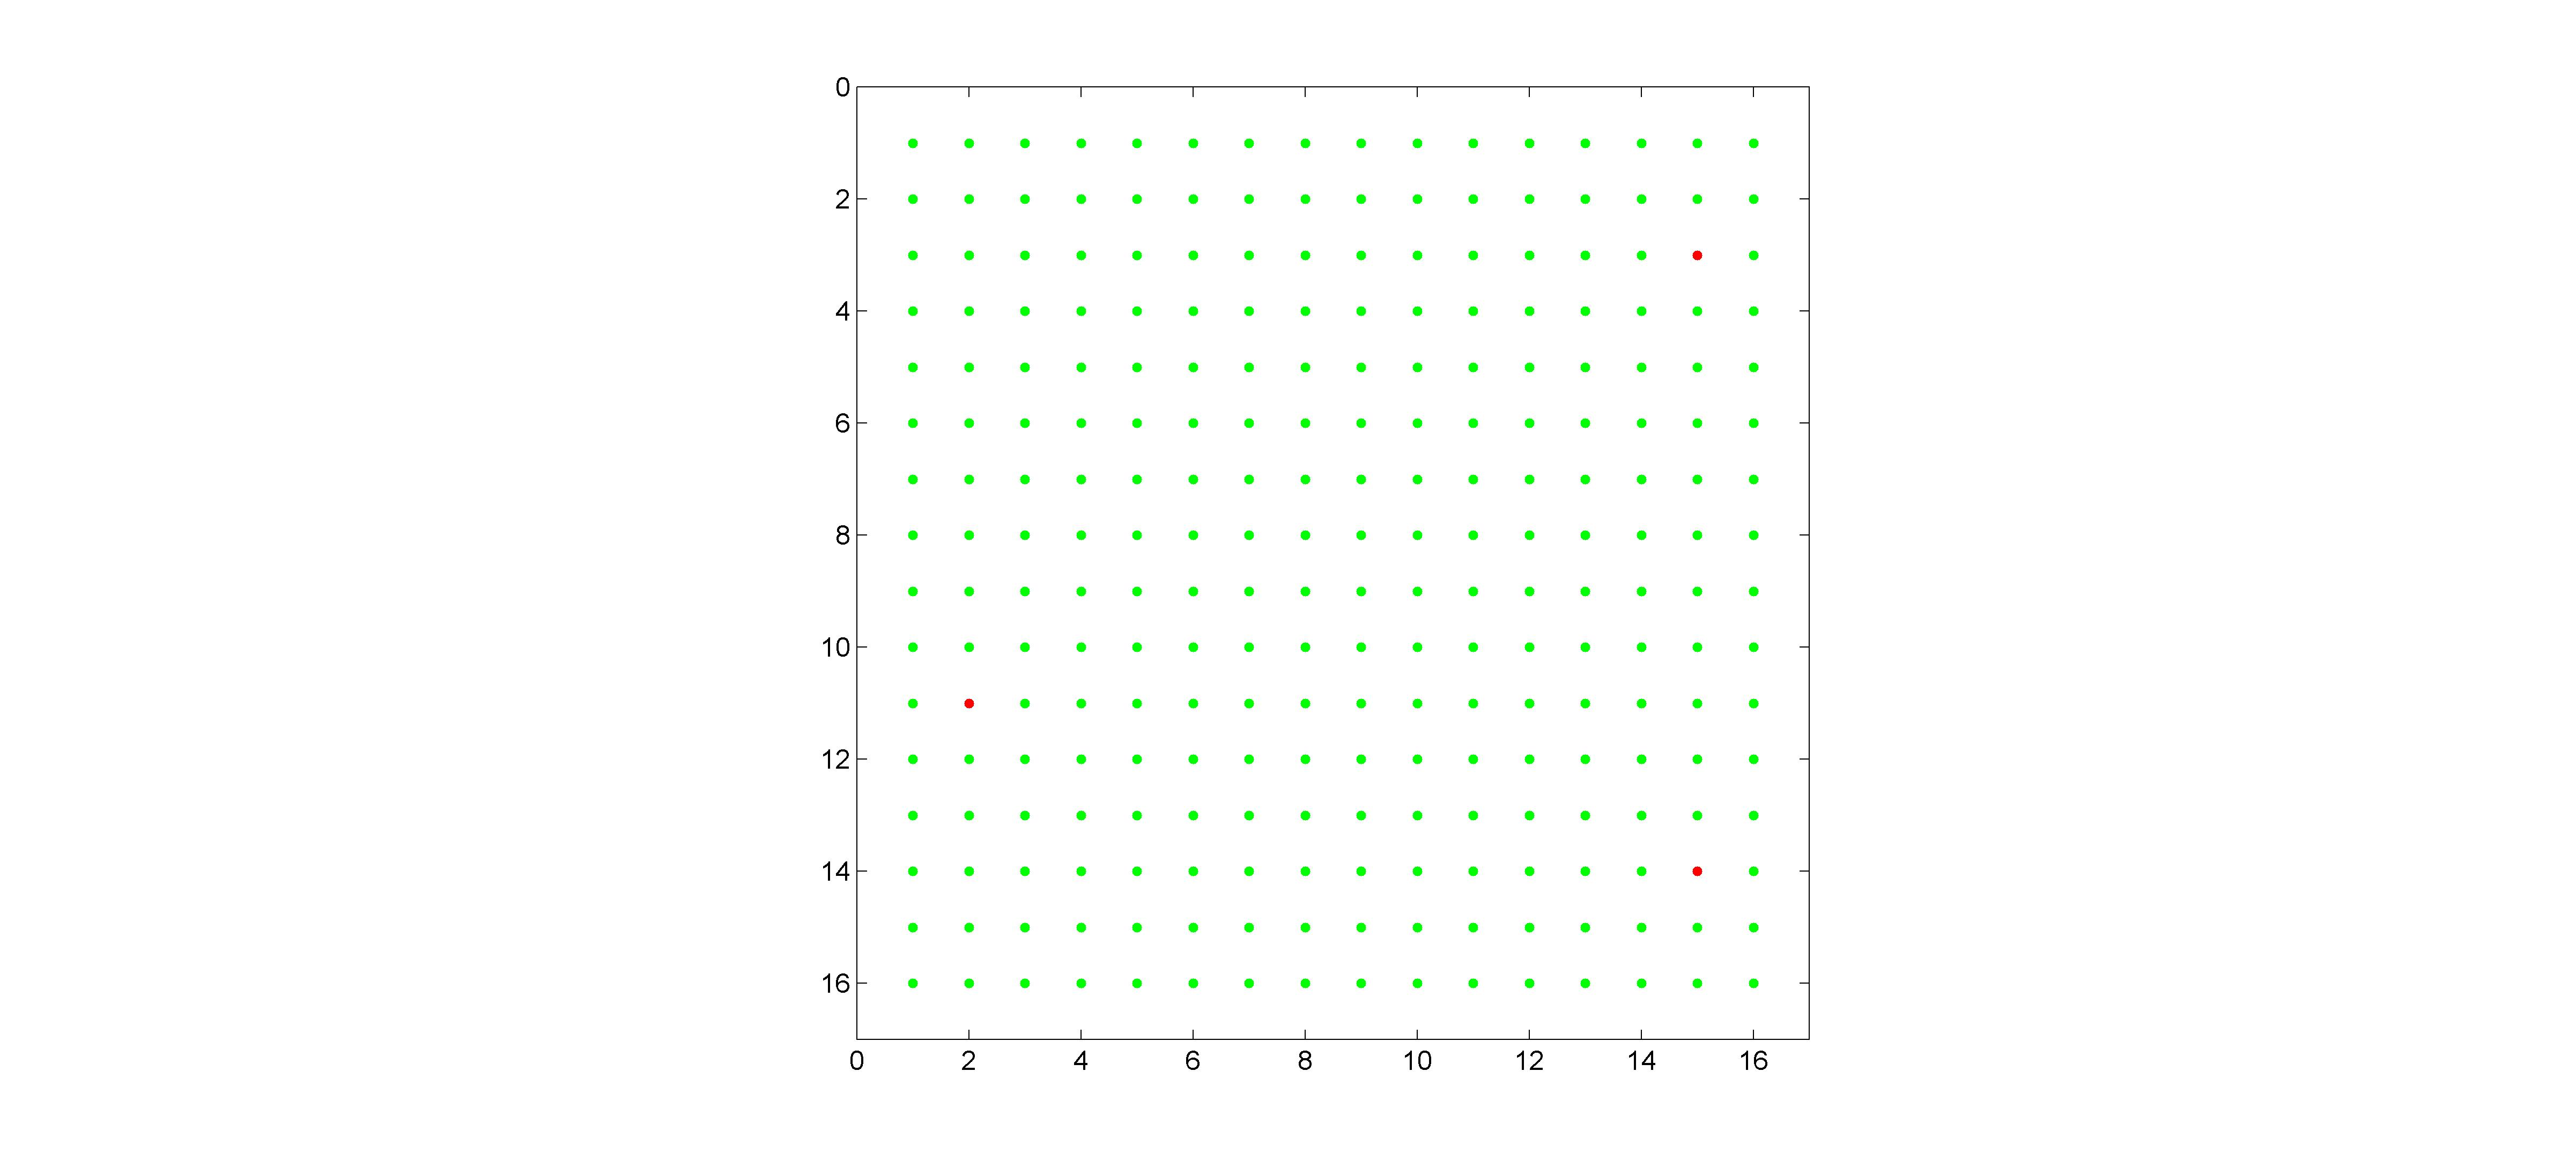
\includegraphics[width=\linewidth]{spice_mat_cmp}
\caption{SPICE与Matlab仿真吻合测试}
\label{fig:spice_mat_cmp}
\end{figure}

所以在 Matlab 中实现 N=4, K=9 的 DBRPUF 仿真。
故根据工艺参数生成1000张网表,带入模型中,给入1000个随机激励,得到一个 $ 1000\times 1000 $ 的 CRP 矩阵。
表\ref{tab:dbr_simu_list}列出了电路参数。
通过式\ref{eq:metric-rand}和式\ref{eq:metric-uniq}计算 DBRPUF 的片内和片间分布。
图\ref{fig:dbrpuf_dist}展示了改进的 DBRPUF 的随机性分布和独特性分布图。

\begin{table}[thb]
\centering
\caption{SMIC 40nm 仿真参数}\label{tab:dbr_simu_list}
\begin{tabular}{ccccc}
\hline
沟道栅长 & NMOS有源区宽度 & PMOS有源区宽度 & 电源电压 & 温度 \\
40 nm   & 130 nm       & 200 nm        & 1.1 V  & 300K \\
\hline
级数N & 每级交换器数K & & &\\
4 & 9 & & &\\
\hline
\end{tabular}
\end{table}


\begin{figure}[htb!]
\centering
\subfloat[随机性]{
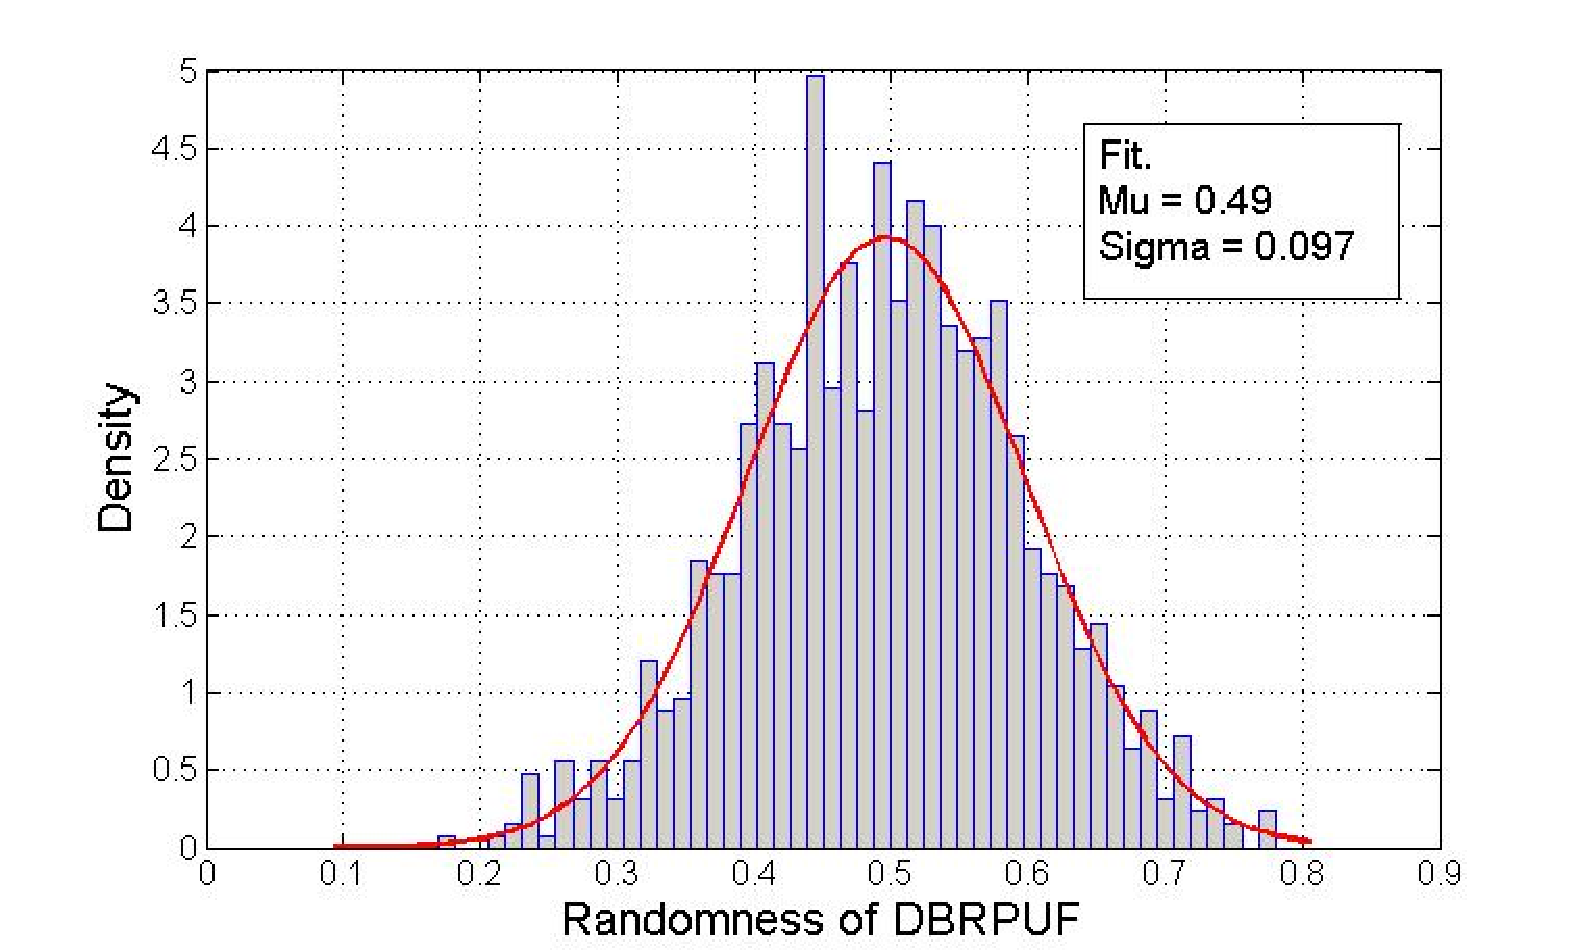
\includegraphics[width=.75\linewidth]{dbrpuf_rand_simulation}
}\\
\subfloat[独特性]{
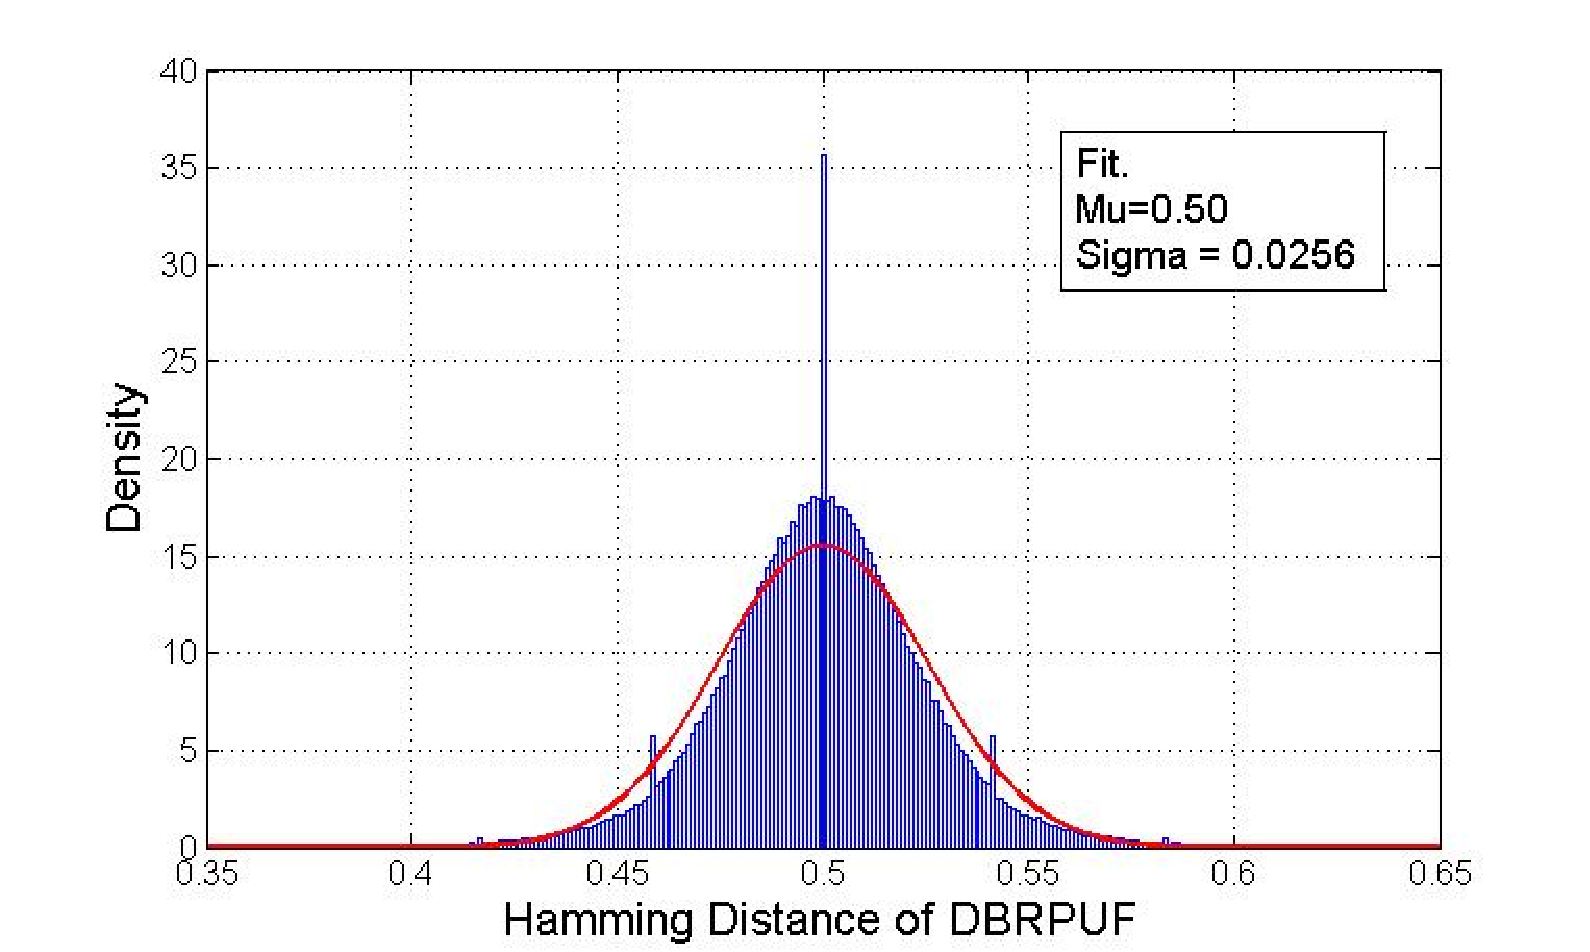
\includegraphics[width=.75\linewidth]{dbrpuf_uniq_simulation}
}
\caption{DBRPUF分布图}
\label{fig:dbrpuf_dist}
\end{figure}

可以看出 DBRPUF 的随机性分布达到 $ N_{rand}\sim(0.49,0.097) $,独特性分布达到 $ N_{uniq}\sim(0.50,0.0256) $,满足上小节的理论分析。相比于 BRPUF 大大改善了输出分布情况。
但是 DBRPUF 的 CRP 仍然是n维空间线性可分,其复杂度与传统仲裁型 PUF 和 BRPUF 相当,为了提高模型复杂度必须采用多 PUF 单元异或的方式,无疑增加了电路的面积功耗开销,不利于 PUF 的实现。


\section{FPGA实现}
采用 Altera Stratix V 芯片,用3块 FPGA 综合并实现 DBRPUF 设计。图\ref{fig:dbrpuf_chipplan}展示了 DBRPUF 实现的 FPGA 版图,我们用一个查找表 (Lookup Table, LUT) 实现交换器,故每一个单元级需要 $ K+2 $ 个 LUT 实现 $ K $ 个交换器和2个与非门。与 BRPUF 一样,需要手动设计 LUT 的摆放位置以保证布线的平衡。
用 Altera Quartus II 中的 LogicLock (逻辑锁定)功能,可以固定节点在版图中的位置。使用 Python 编写了自动布局脚本,用多叉树数据结构实现了按模块关系自动排列。

读出逻辑采用 250 MHz 时钟连续采样,考虑到环路振荡需要一定的稳定时间,若在 1000 个时钟周期内存在100个连续稳定的值则视其为输出,保存在输出寄存器中。
寄存器的值和控制逻辑通过 PCI-E 接口与 PC 相连。在 PC 端单独开辟一块2 GB 内存空间用于存放 CRP, 最后通过 C 程序直接读出内存中的数值。


\begin{figure}[htb]
\centering
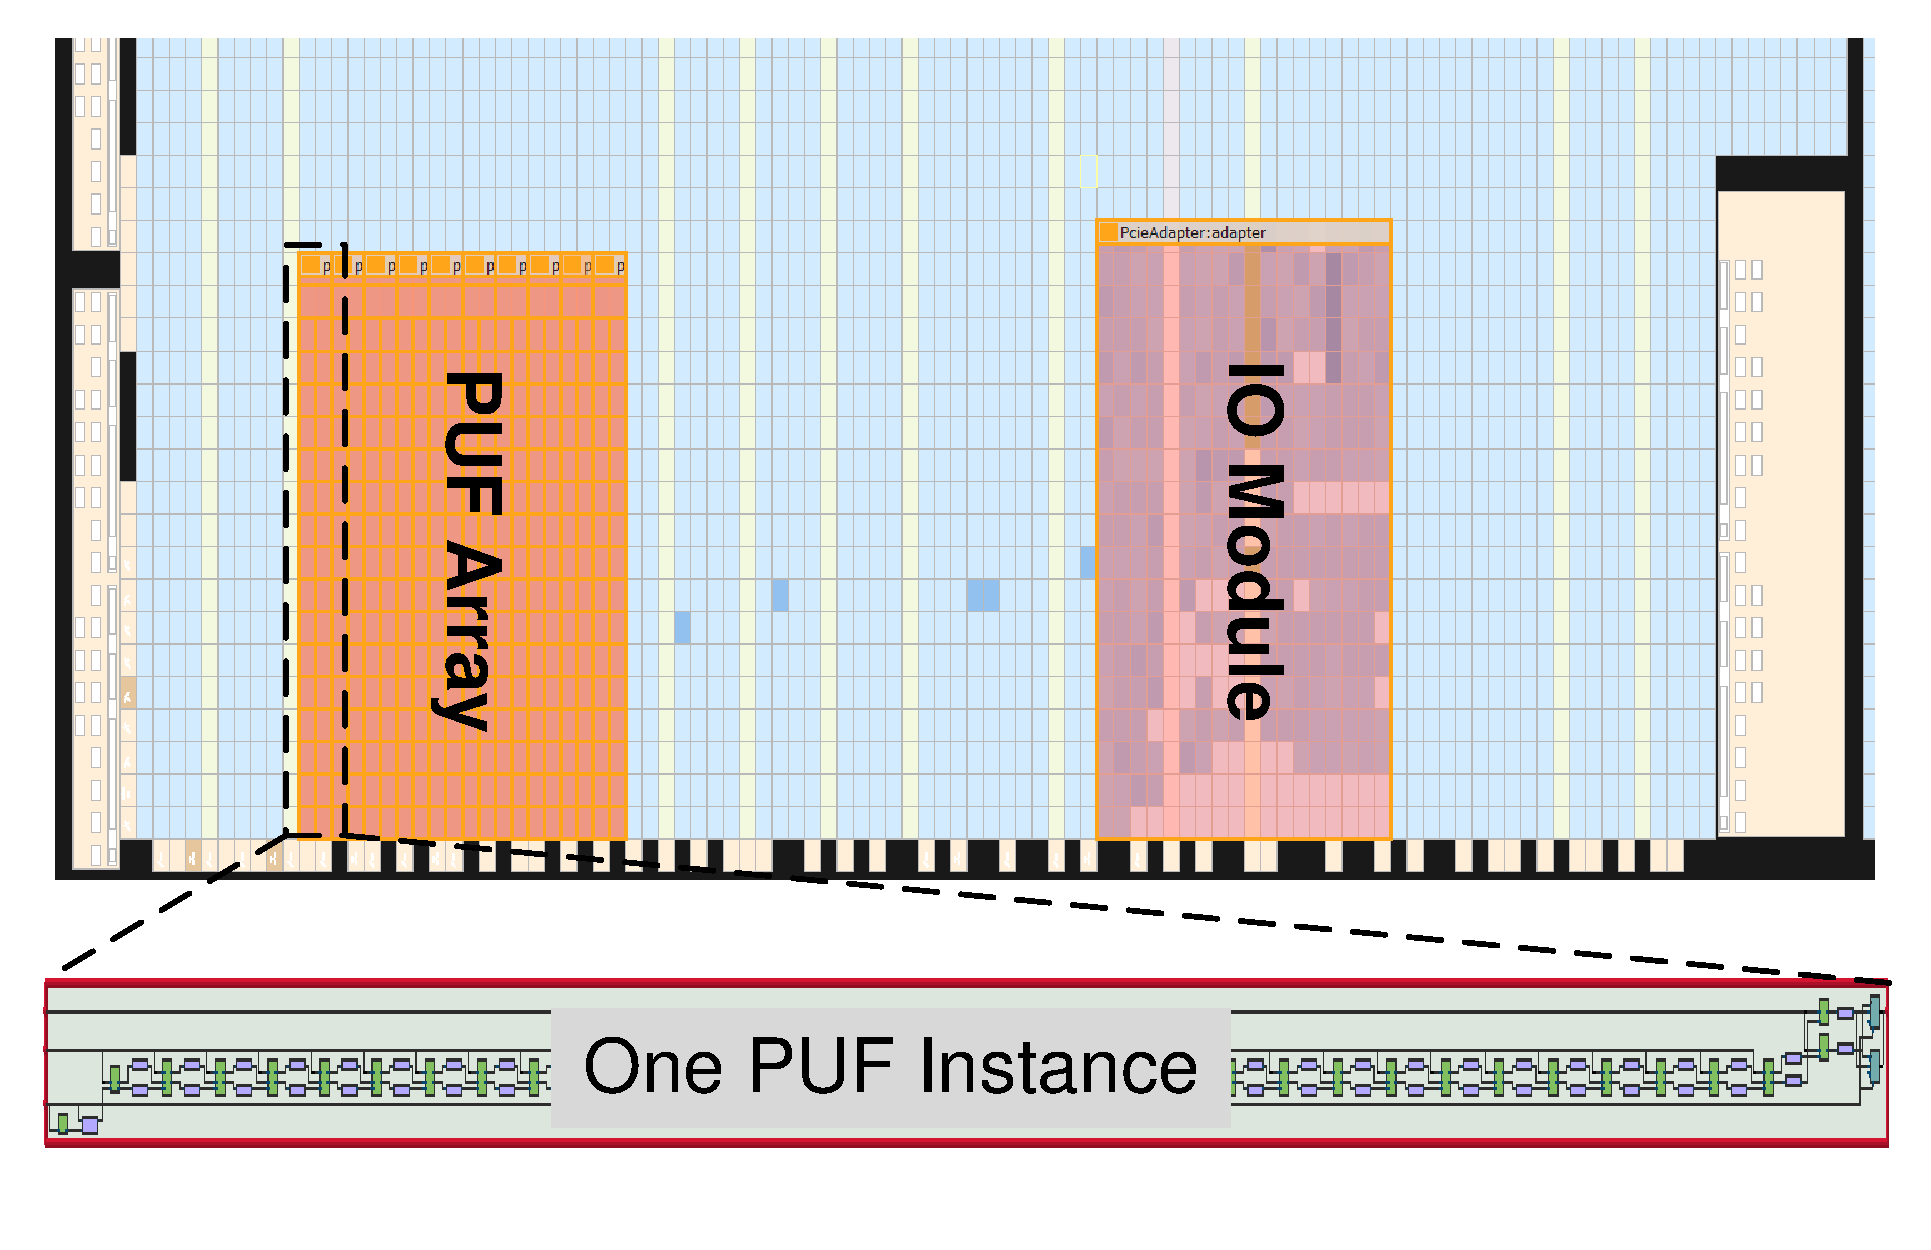
\includegraphics[width=.8\linewidth]{dbrpuf_cp}
\caption{DBRPUF在FPGA的Chipplan示意图}
\label{fig:dbrpuf_chipplan}
\end{figure}

\begin{figure}[htb]
\centering
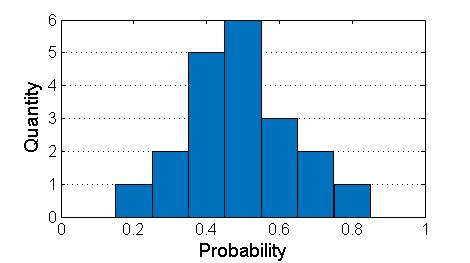
\includegraphics[width=.8\linewidth]{dbrpuf_rand_fpga}
\caption{FPGA 上 DBRPUF 随机性分布统计}
\label{fig:dbr_rand}
\end{figure}

在每块 FPGA 芯片的不同位置摆下10个 DBRPUF,共享一个读出逻辑,一共30个独立 PUF 元件。
控制 FPGA 的电源电压为1.5 V,
温度处于室温环境。
每个 PUF 等概率给予5000个随机32位激励,每个激励重复100次以验证可重复性,记录输出寄存器共 $ 30\times 5000\times 100 $ 个输出,经过 Matlab 统计分析,得到 DBRPUF 的随机性、独特性和可靠性分布。如图\ref{fig:dbr_rand},图\ref{fig:dbrpuf_dist_fpga}所示, DBRPUF 的独特性满足 $ N\sim(0.494,0.0048) $ 的高斯分布,可靠性满足 $ N\sim(0.057,0.013) $ 的高斯分布(随机性样本太少不做统计)。

\begin{figure}[htb!]
\centering
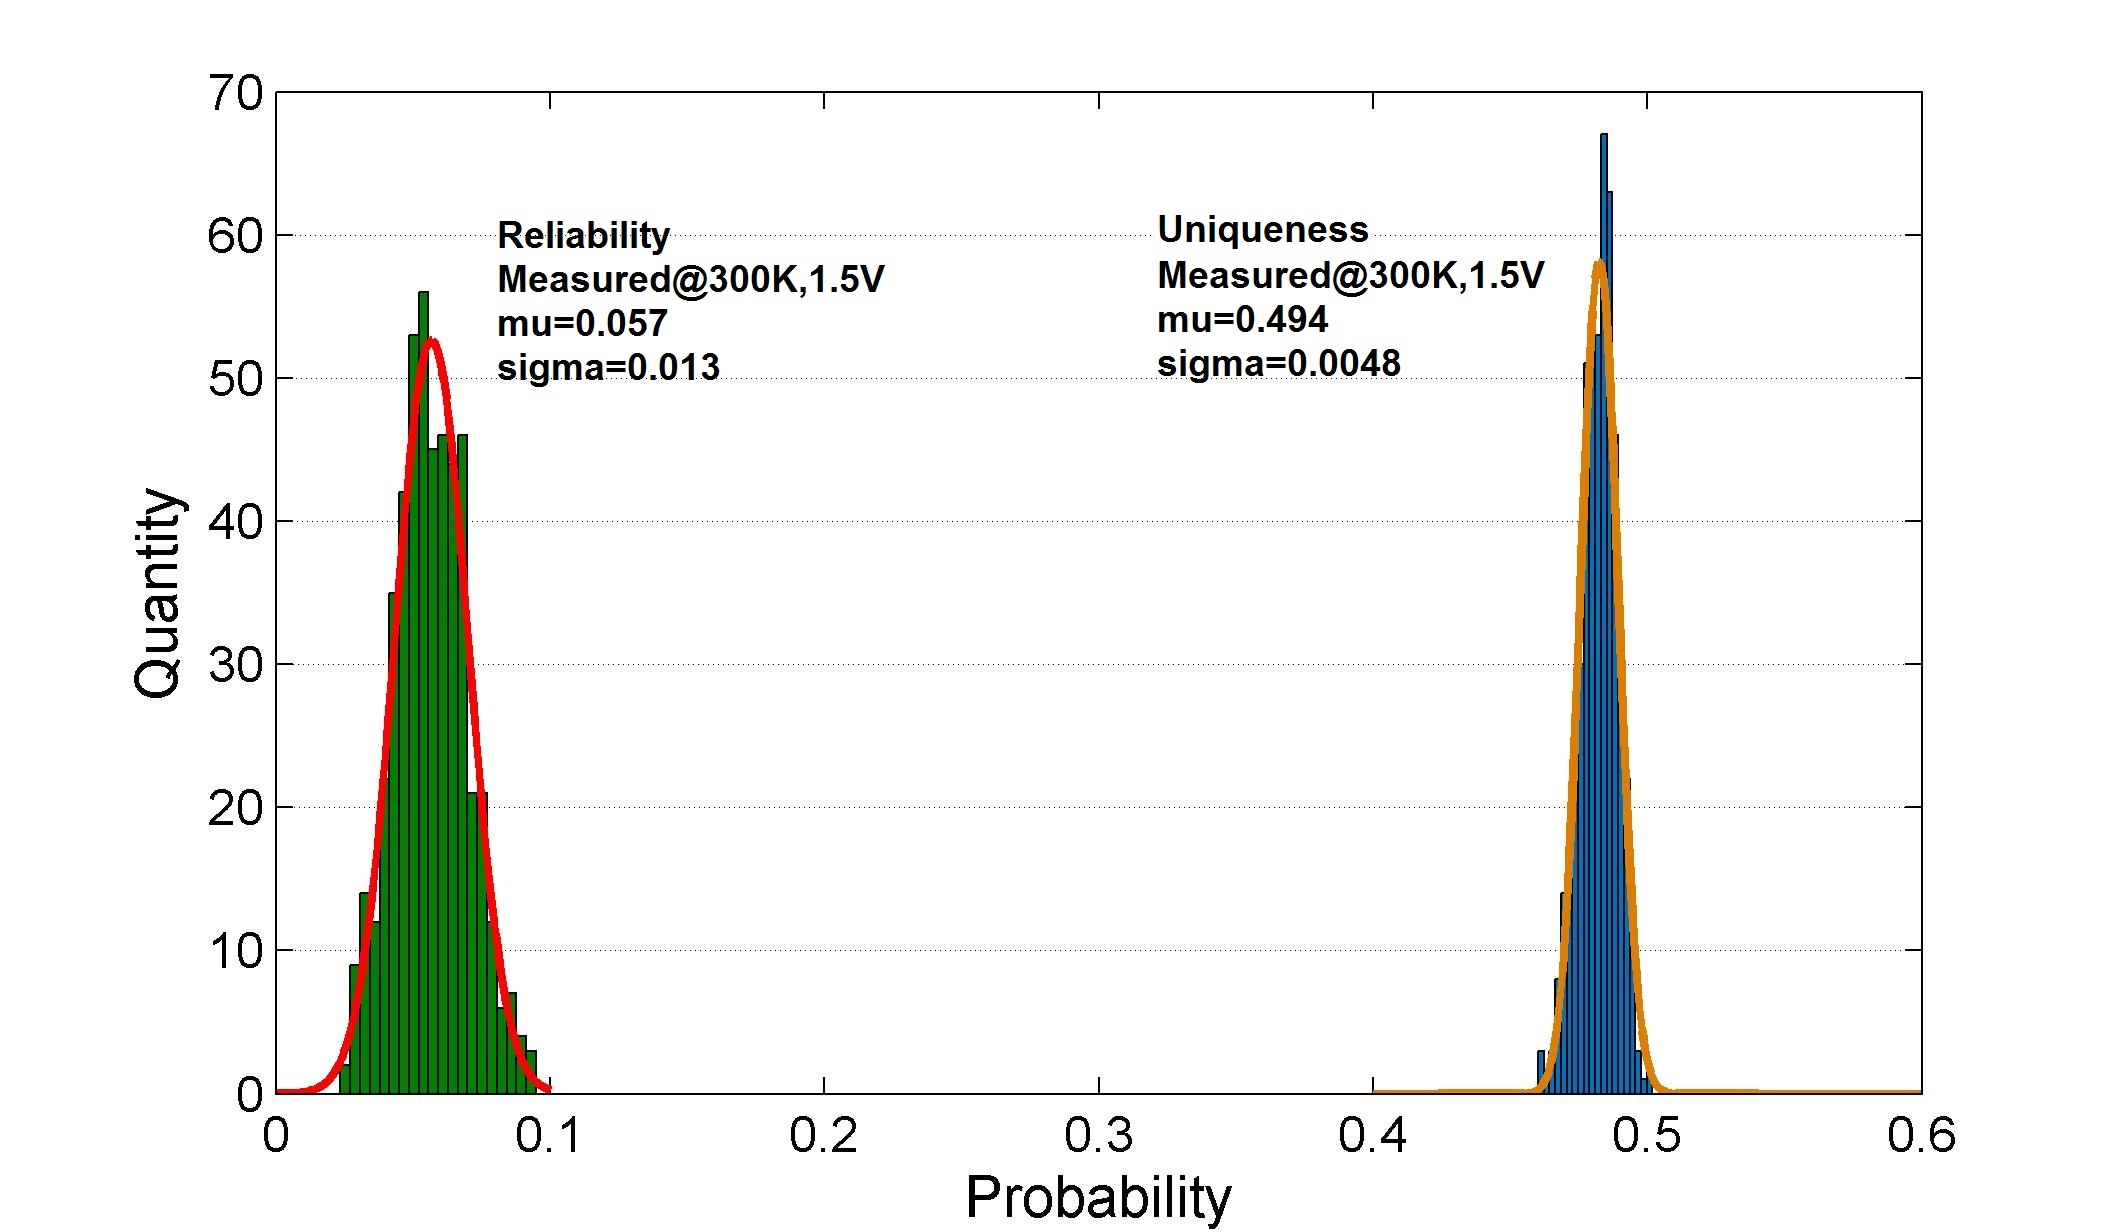
\includegraphics[width=.8\linewidth]{dbrpuf_uniq_fpga}
\caption{FPGA 上 DBRPUF 独特性和可靠性统计分布}
\label{fig:dbrpuf_dist_fpga}
\end{figure}

可以看出 DBRPUF 的统计分布优于 BRPUF。在\ref{chap:rpapuf}章中将对 DBRPUF 进行 NIST 测试和建模攻击,结果参见\ref{sec:rpa_summary}。

\section{本章小结}
本章基于 BRPUF 和交换器设计了一种新型 PUF 结构,称为延迟双稳环路 PUF ( Delay-based Bistable Ring PUF )。
DBRPUF 改善了 BRPUF 分布分散的缺点,使得统计特性比 BRPUF 更好。并且从理论、仿真与 FPGA 实现三方面验证了这一结论。

但 DBRPUF 相比于传统仲裁型 PUF 并没有显著优势,其分布结果也没有达到最理想的效果,从模型复杂度来看,DBRPUF 的最小线性可分空间同样为N,说明建模攻击代价与传统 PUF(仲裁型,双稳态)相当。
